Before implementing the method discussed above to planar graphs, we first investigate Ricci curvature flow on three types of simple graphs: a stochastic block model (SBM) graph, a Barbell graph, and a Caveman graph. Each graph type exhibits distinct structural properties, facilitating a comprehensive exploration of Ricci flow dynamics.

\section{\textit{GraphRicciCurvature} Library}
In addition to the main library for networks, \textit{Networkx}, the developed code relies on the \textit{GraphRicciCurvature} library, which provides efficient algorithms for calculating the Ollivier-Ricci curvature on graphs.

Key features of the \textit{GraphRicciCurvature} library include:

\begin{itemize}
    \item \textbf{OllivierRicci Class}: This class is initialized with the graph and a parameter \texttt{alpha}, which controls the curvature's sensitivity to edge weights. Smaller alpha values (closer to 0) are often used when one focuses on local community detection, small subgraphs, or clusters. Larger alpha values (closer to 1) are used when the interest is in the global structure of the graph, such as long-range connections and global topology.
    
    \item \textbf{Curvature Computation}: The method \texttt{compute\_ricci\_curvature()} calculates the Ricci curvature for all edges in the graph.
    
    \item \textbf{Edge Curvature Assignment}: After computing the curvatures, the edge attributes of the original graph are updated with the curvature values calculated by the \texttt{OllivierRicci} instance. 
\end{itemize}



\section{Results}

The Ricci Flow method was tested on three different types of graphs to evaluate its functionalities and performance. Each graph has distinct structural properties, making them ideal candidates for assessing the method’s ability to identify both densely connected intra-community edges and sparser inter-community edges. For each graph type the Ricci Flow process has been simulated using 15 iterations and an alpha of 0.5. The results are summarized below. 

\textbf{Stochastic Block Model (SBM) graph}: This graph is specifically designed to simulate community structures with predefined groups. Nodes within the same group are more likely to connect, while connections between groups are less frequent. We created an SBM graph with two communities of 50 nodes each, where the intra-community edge probability was set high to ensure clear separation between the communities. The Ricci Flow method (with threshold for surgery set to -0.05) successfully identified the two distinct communities, as illustrated in Figure \hyperref[fig2]{2}.

\textbf{Barbell graph}: The barbell graph consists of two complete graphs (dense communities) connected by a path (sparse inter-community links). It is an excellent test case for methods that detect clear community boundaries with sparse connections between them. In our experiments, we used a barbell graph with two communities of 20 nodes each, connected by a 5-node path. The method  (with threshold for surgery set to -0.1) correctly detected the two communities, with the inter-community path clearly stretched due to the low curvature, as seen in Figure \hyperref[fig3]{3}.

\textbf{Caveman graph}: A caveman graph is another community-like structure where several cliques (complete subgraphs) are loosely connected. This type of graph is useful for testing models aimed at detecting clique-based communities. We tested the method on a caveman graph with 5 cliques, each consisting of 10 nodes. The method (with threshold for surgery set to 0) successfully separated the cliques, identifying each as a distinct community, as shown in Figure \hyperref[fig4]{4}.

Across all three graph types, the developed Ricci Flow-based method behaved as expected, demonstrating its capability to detect both dense and sparse community structures. The method shrank intra-community edges and stretched inter-community edges, which aligns with the behavior predicted by the underlying theory of Ollivier-Ricci curvature. The results from the tests on the SBM graph, Barbell graph, and Caveman graph are displayed in Figures \hyperref[fig2]{2}, \hyperref[fig3]{3}, and \hyperref[fig4]{4} respectively; edges with different colours belong to different communities. 

Additional results and details, such as plots of the networks after Ricci Flow and after surgery,  can be found on the project's GitHub page.


\begin{figure}[h]
    \centering
    \begin{subfigure}[b]{0.45\textwidth}
        \centering
        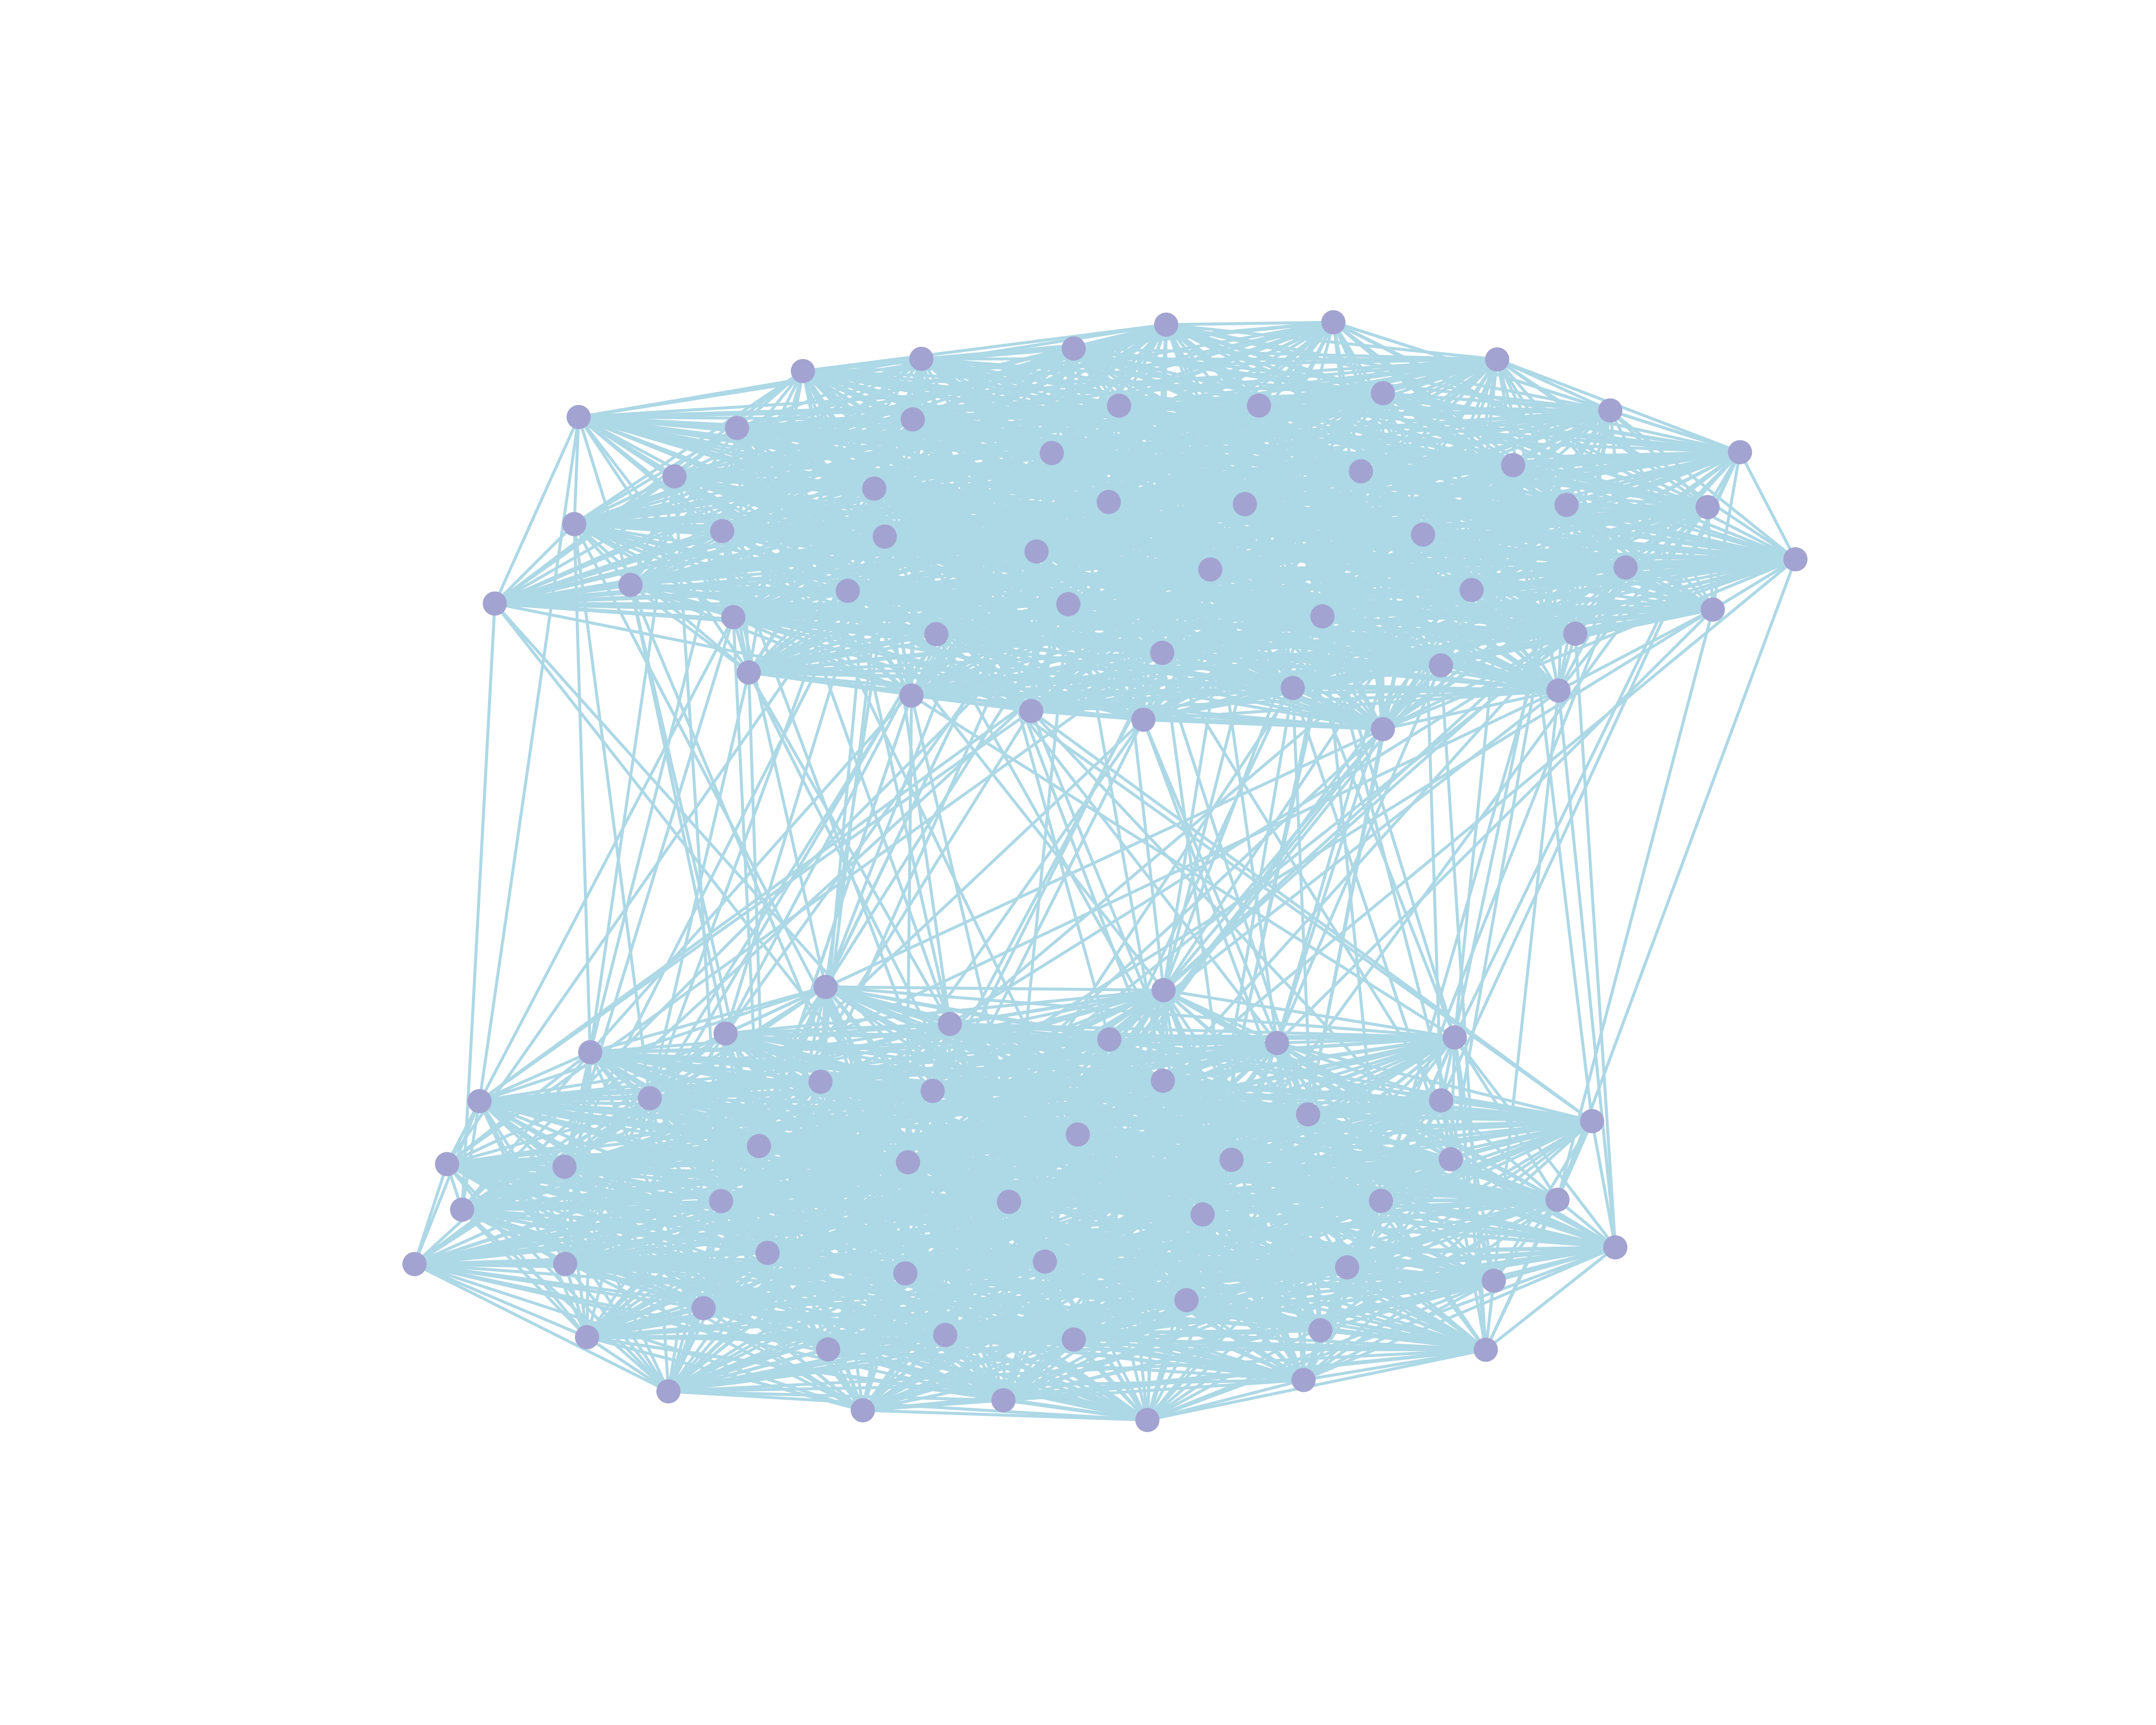
\includegraphics[width=\textwidth]{Graphics/ToyModelResults/SBM_results/BeforeRicciFlow.png}
        \caption{Initial SBM graph}
        \label{fig:sbm_initial}
    \end{subfigure}
    \hfill
    \begin{subfigure}[b]{0.45\textwidth}
        \centering
        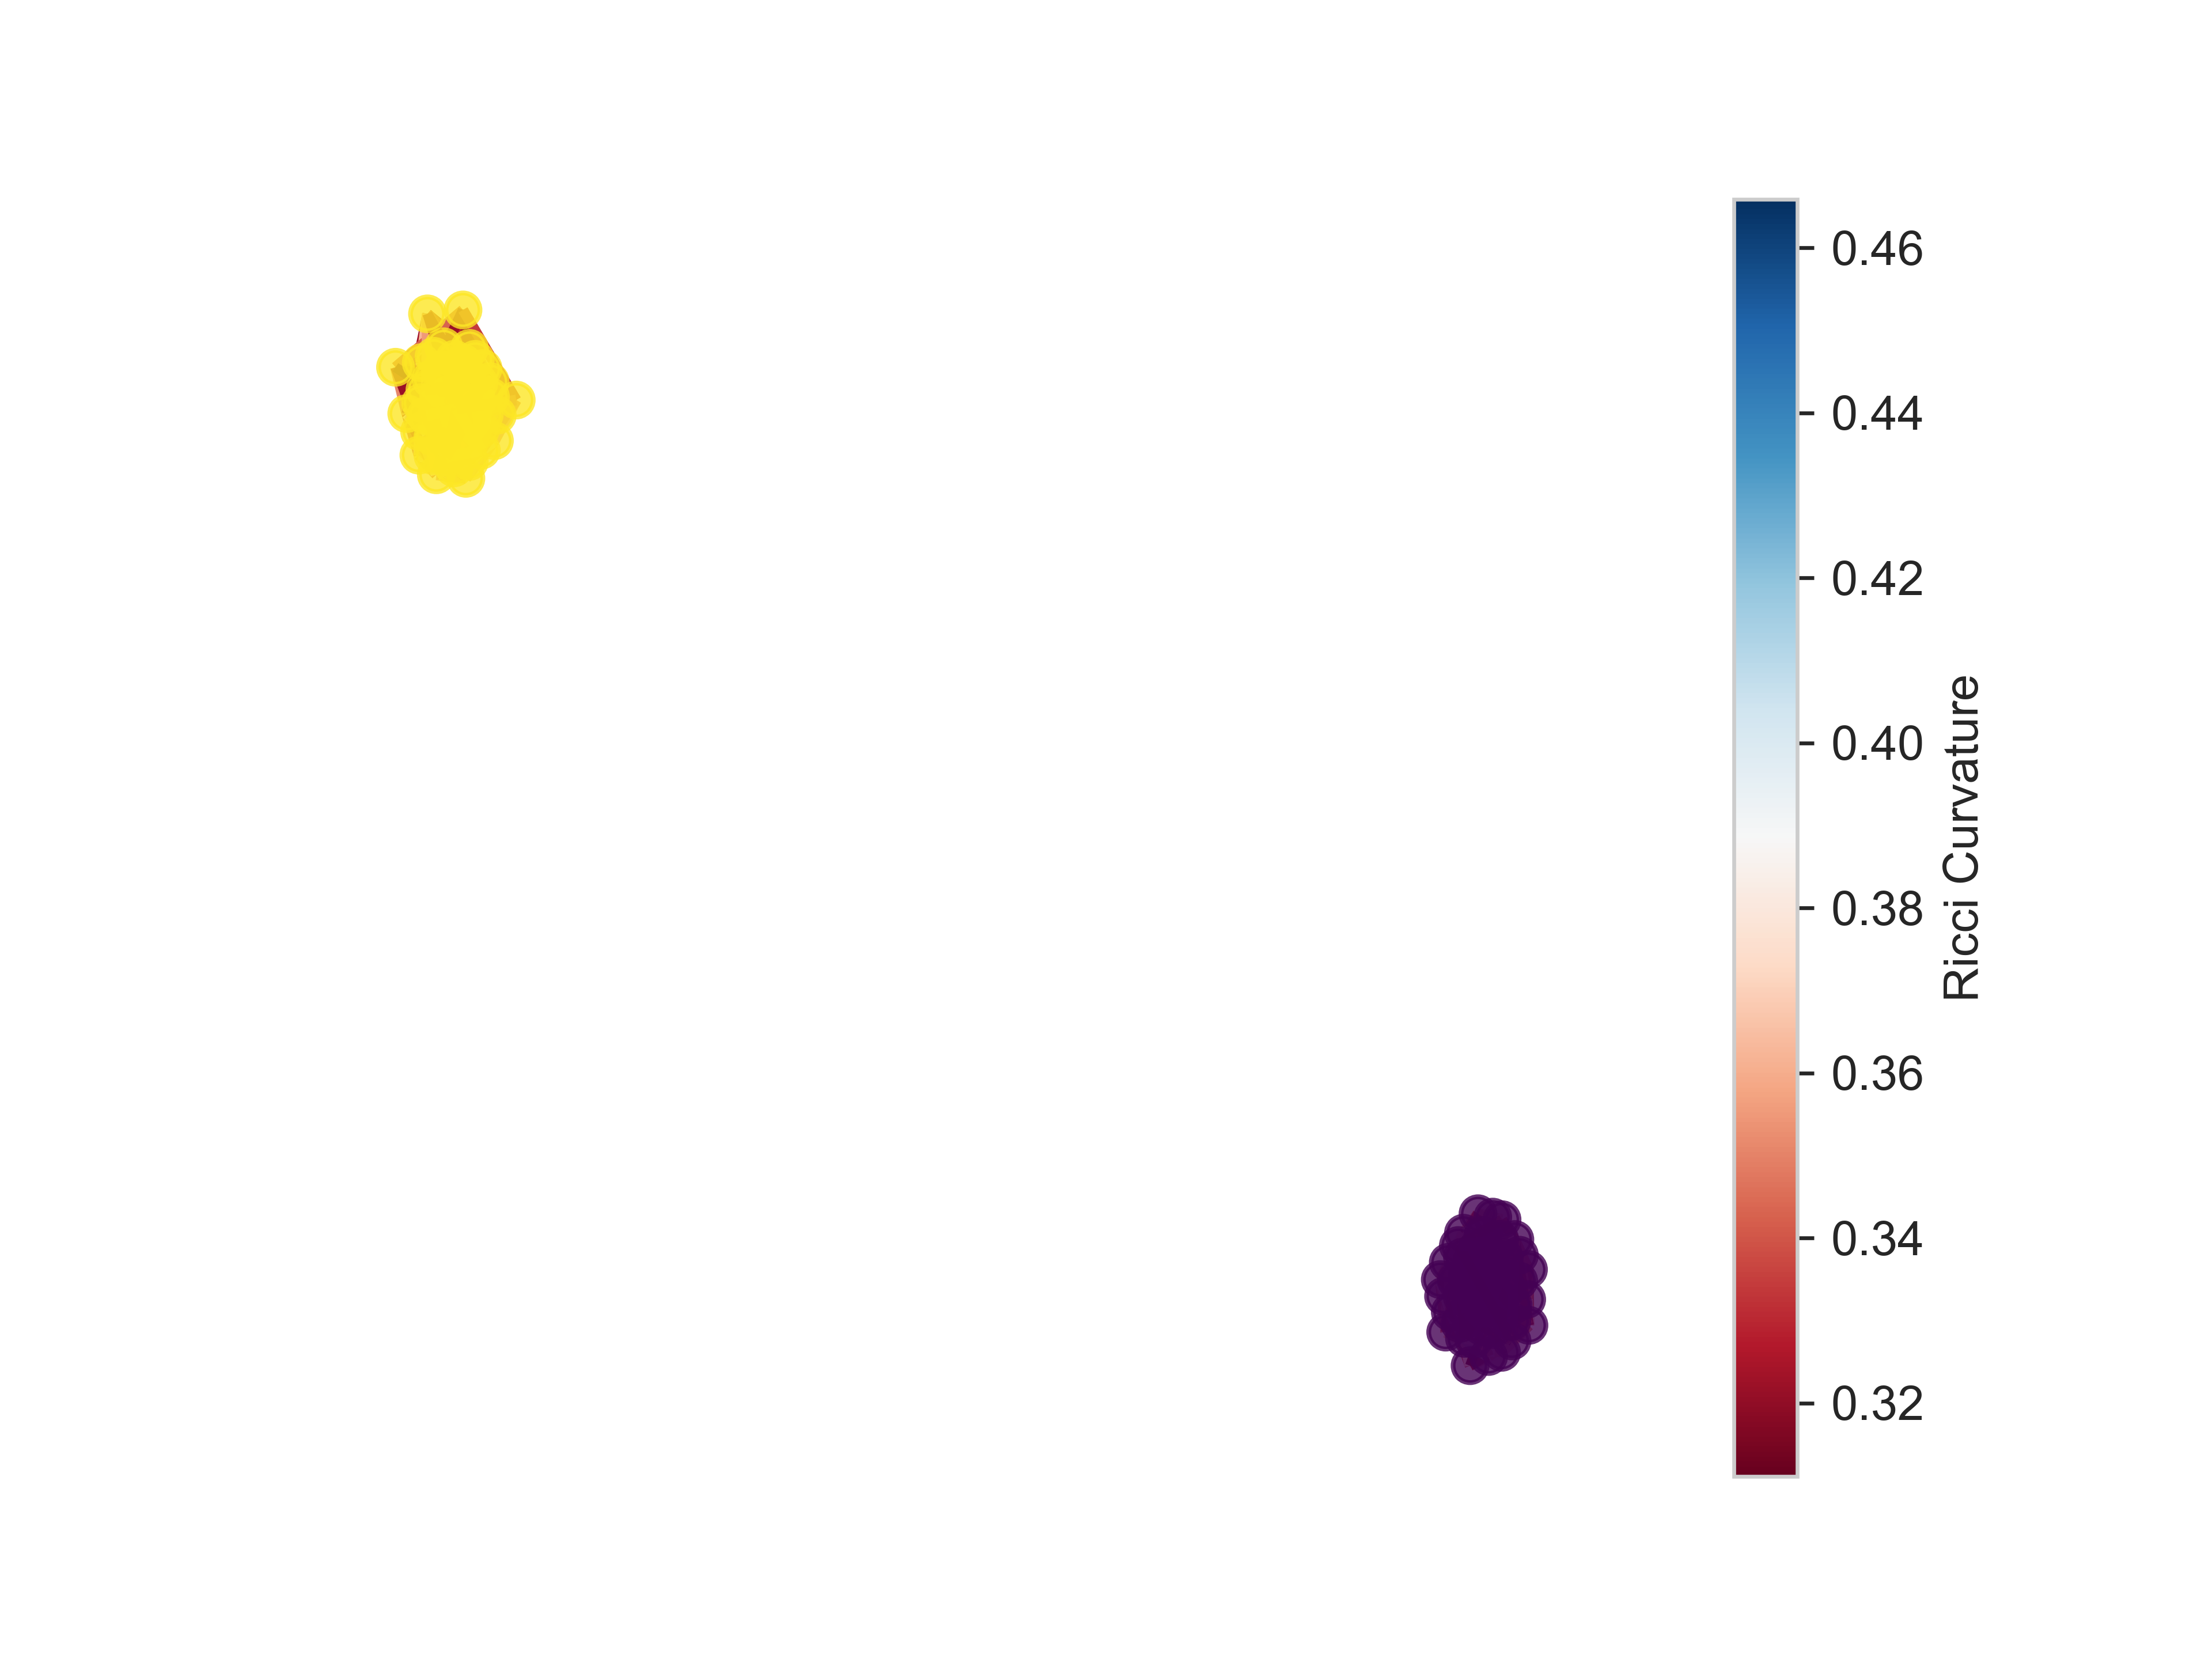
\includegraphics[width=\textwidth]{Graphics/ToyModelResults/SBM_results/Communities.png}
        \caption{Detected communities.}
        \label{fig:sbm_result}
    \end{subfigure}
    \caption{Comparison of the initial SBM graph and the community detection result.}
    \label{fig2}
\end{figure}

\begin{figure}[ht]
    \centering
    \begin{subfigure}[b]{0.45\textwidth}
        \centering
        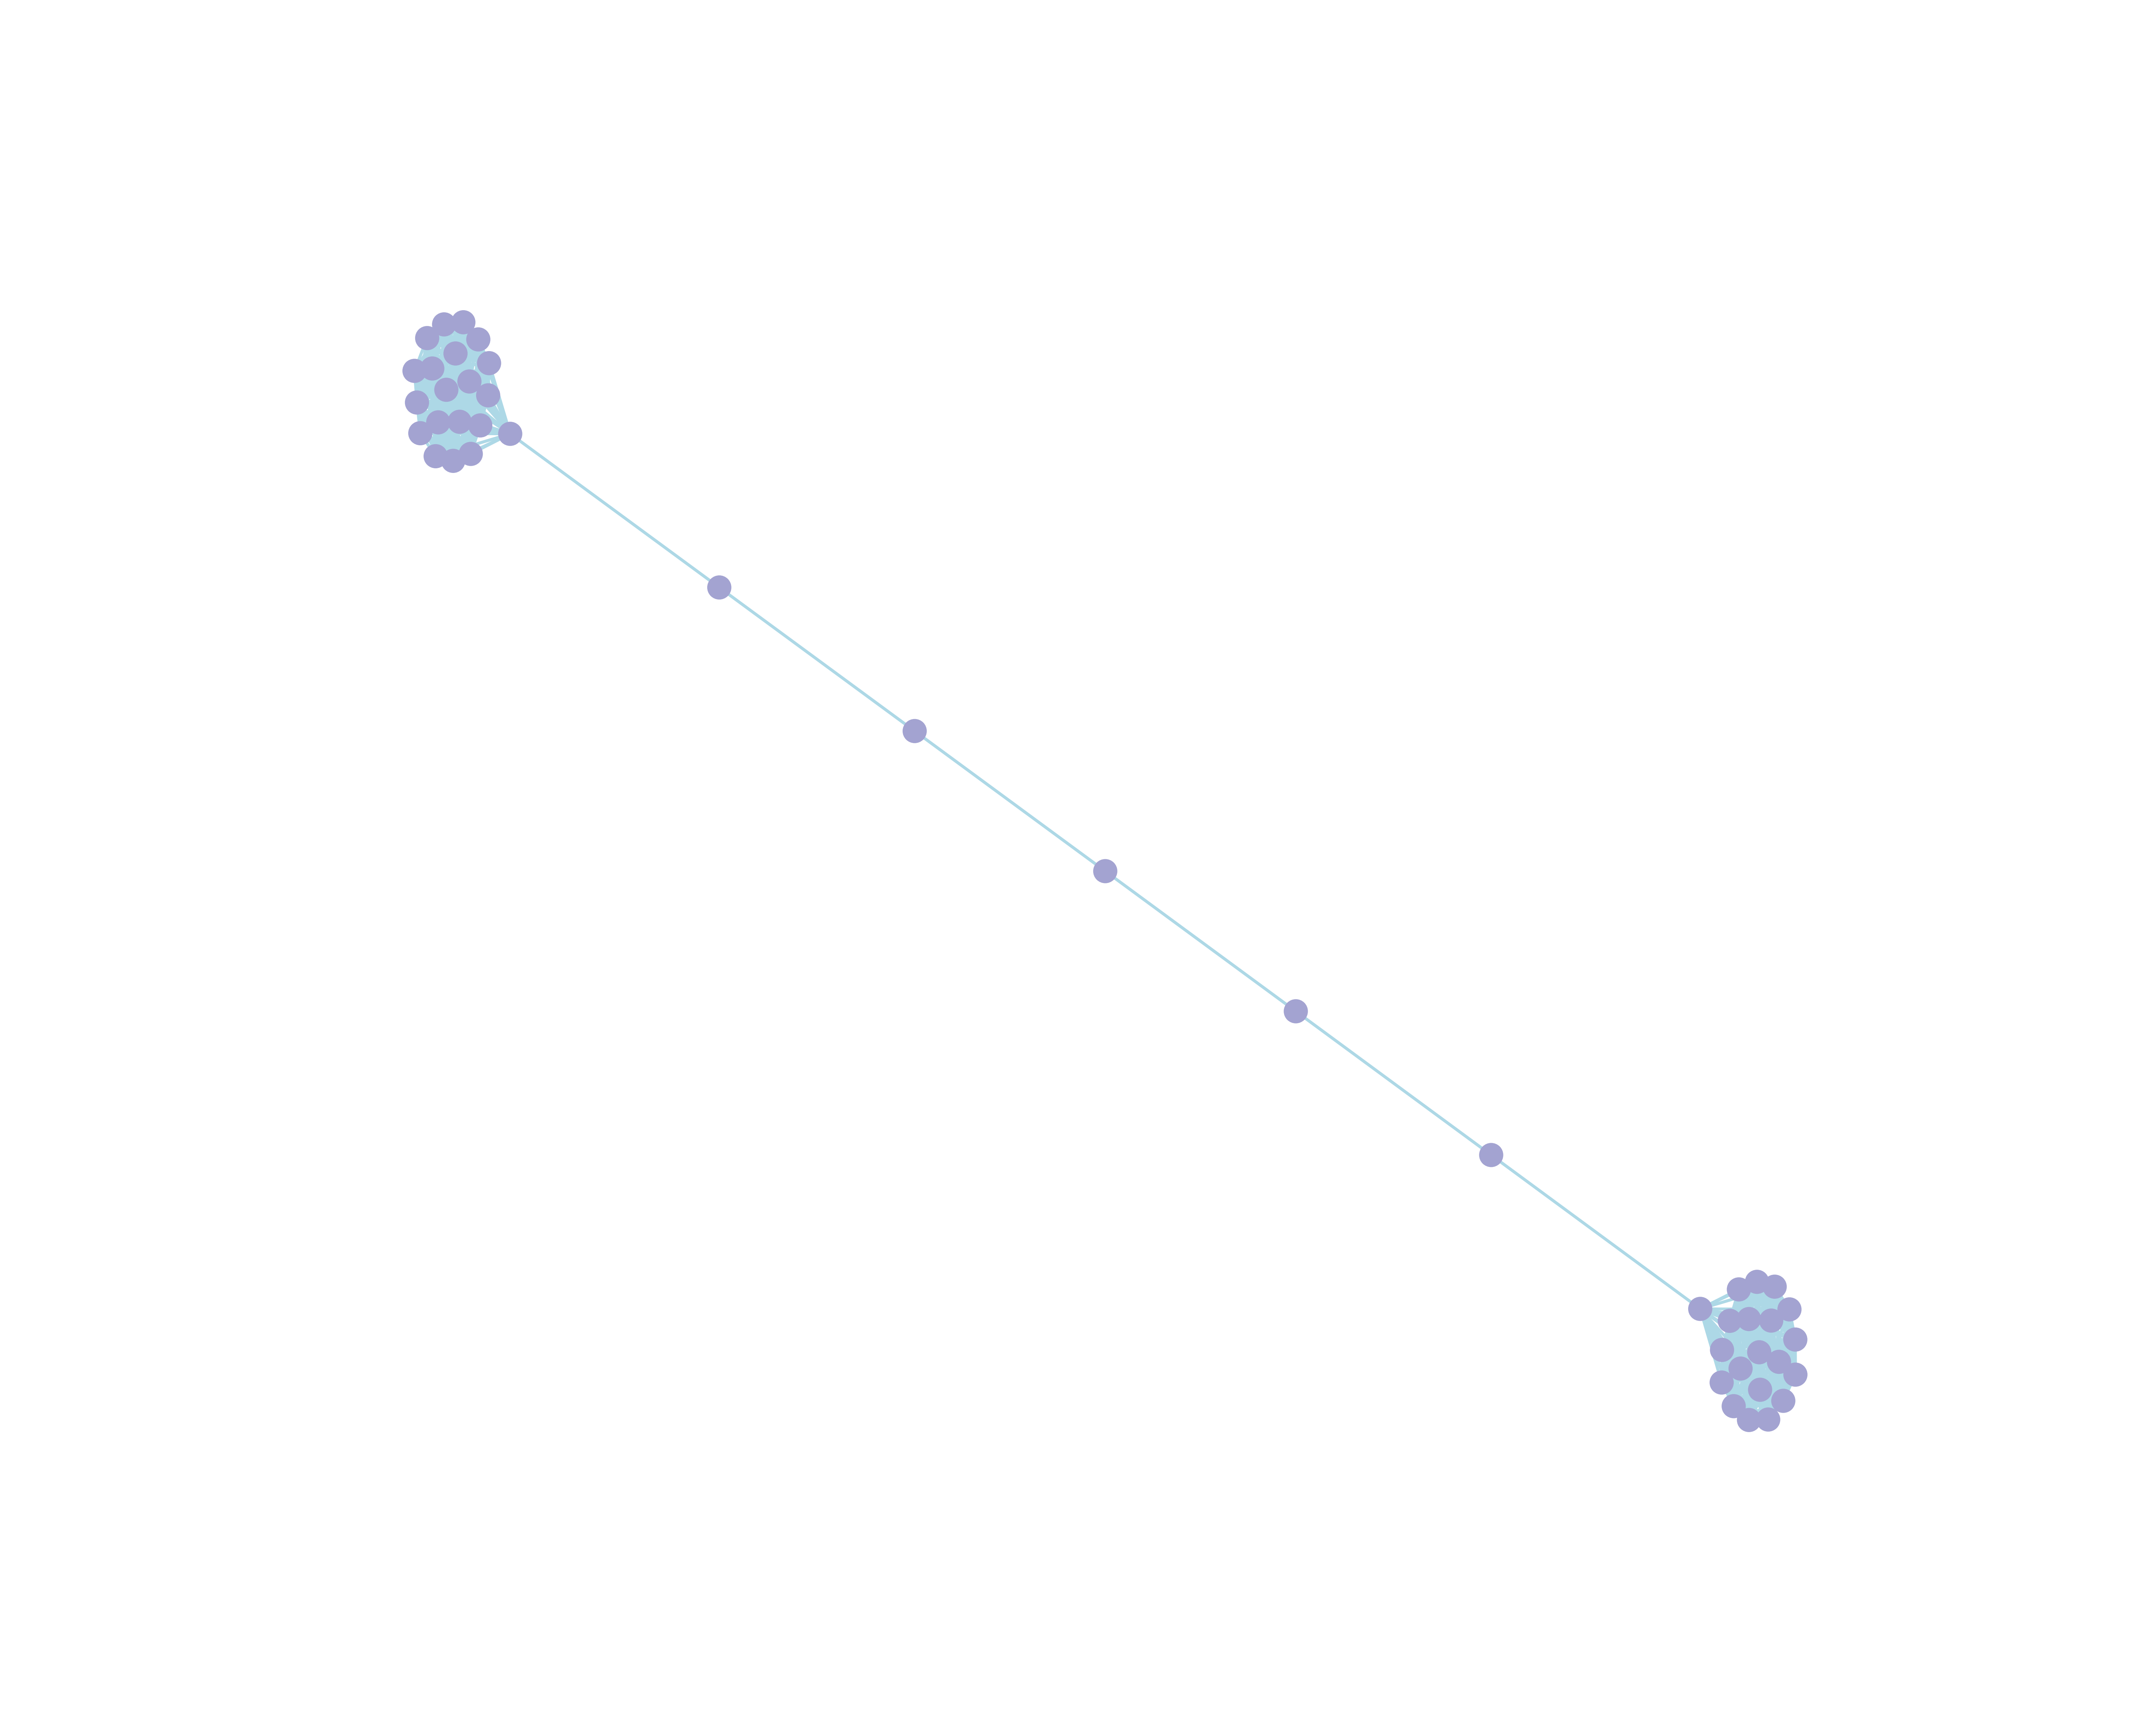
\includegraphics[width=\textwidth]{Graphics/ToyModelResults/Barbell_resluts/BeforeRicciFlow.png}
        \caption{Initial Barbell graph}
        \label{fig:barbell_initial}
    \end{subfigure}
    \hfill
    \begin{subfigure}[b]{0.45\textwidth}
        \centering
        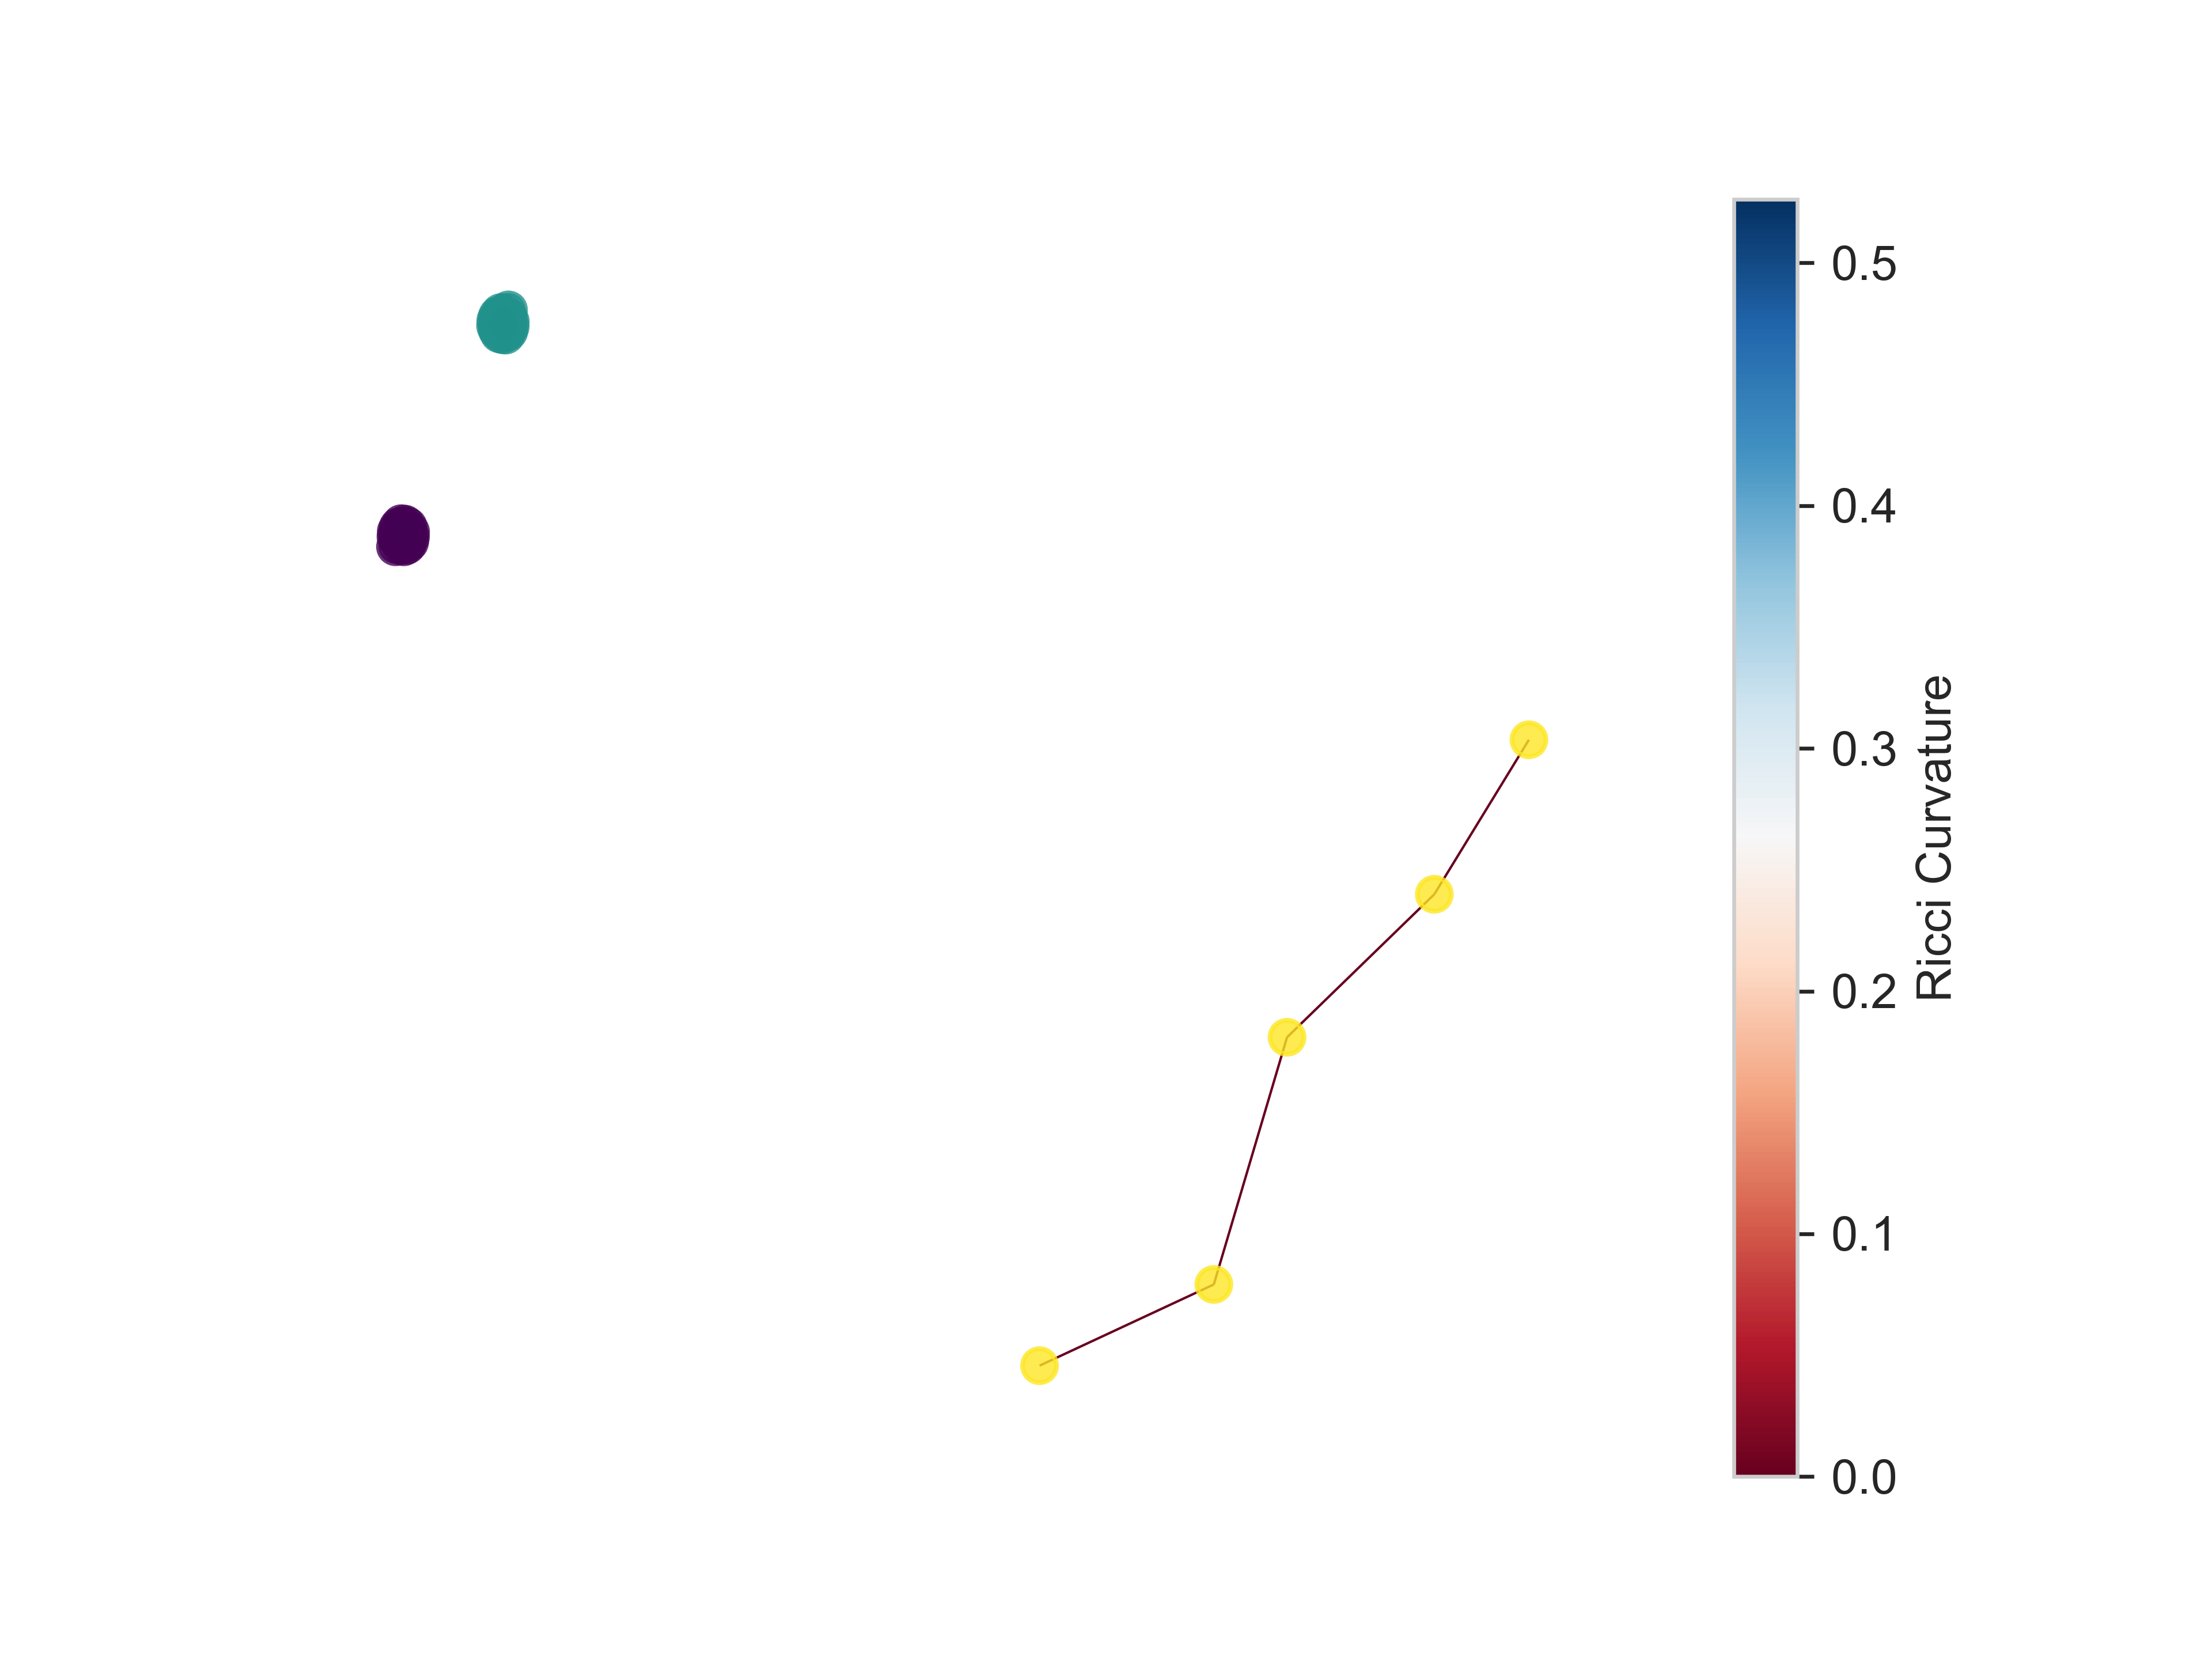
\includegraphics[width=\textwidth]{Graphics/ToyModelResults/Barbell_resluts/Communities.png}
        \caption{Detected communities}
        \label{fig:barbell_result}
    \end{subfigure}
    \caption{Comparison of the initial Barbell graph and the community detection result.}
    \label{fig3}
\end{figure}

\begin{figure}[ht!]
    \centering
    \begin{subfigure}[b]{0.45\textwidth}
        \centering
        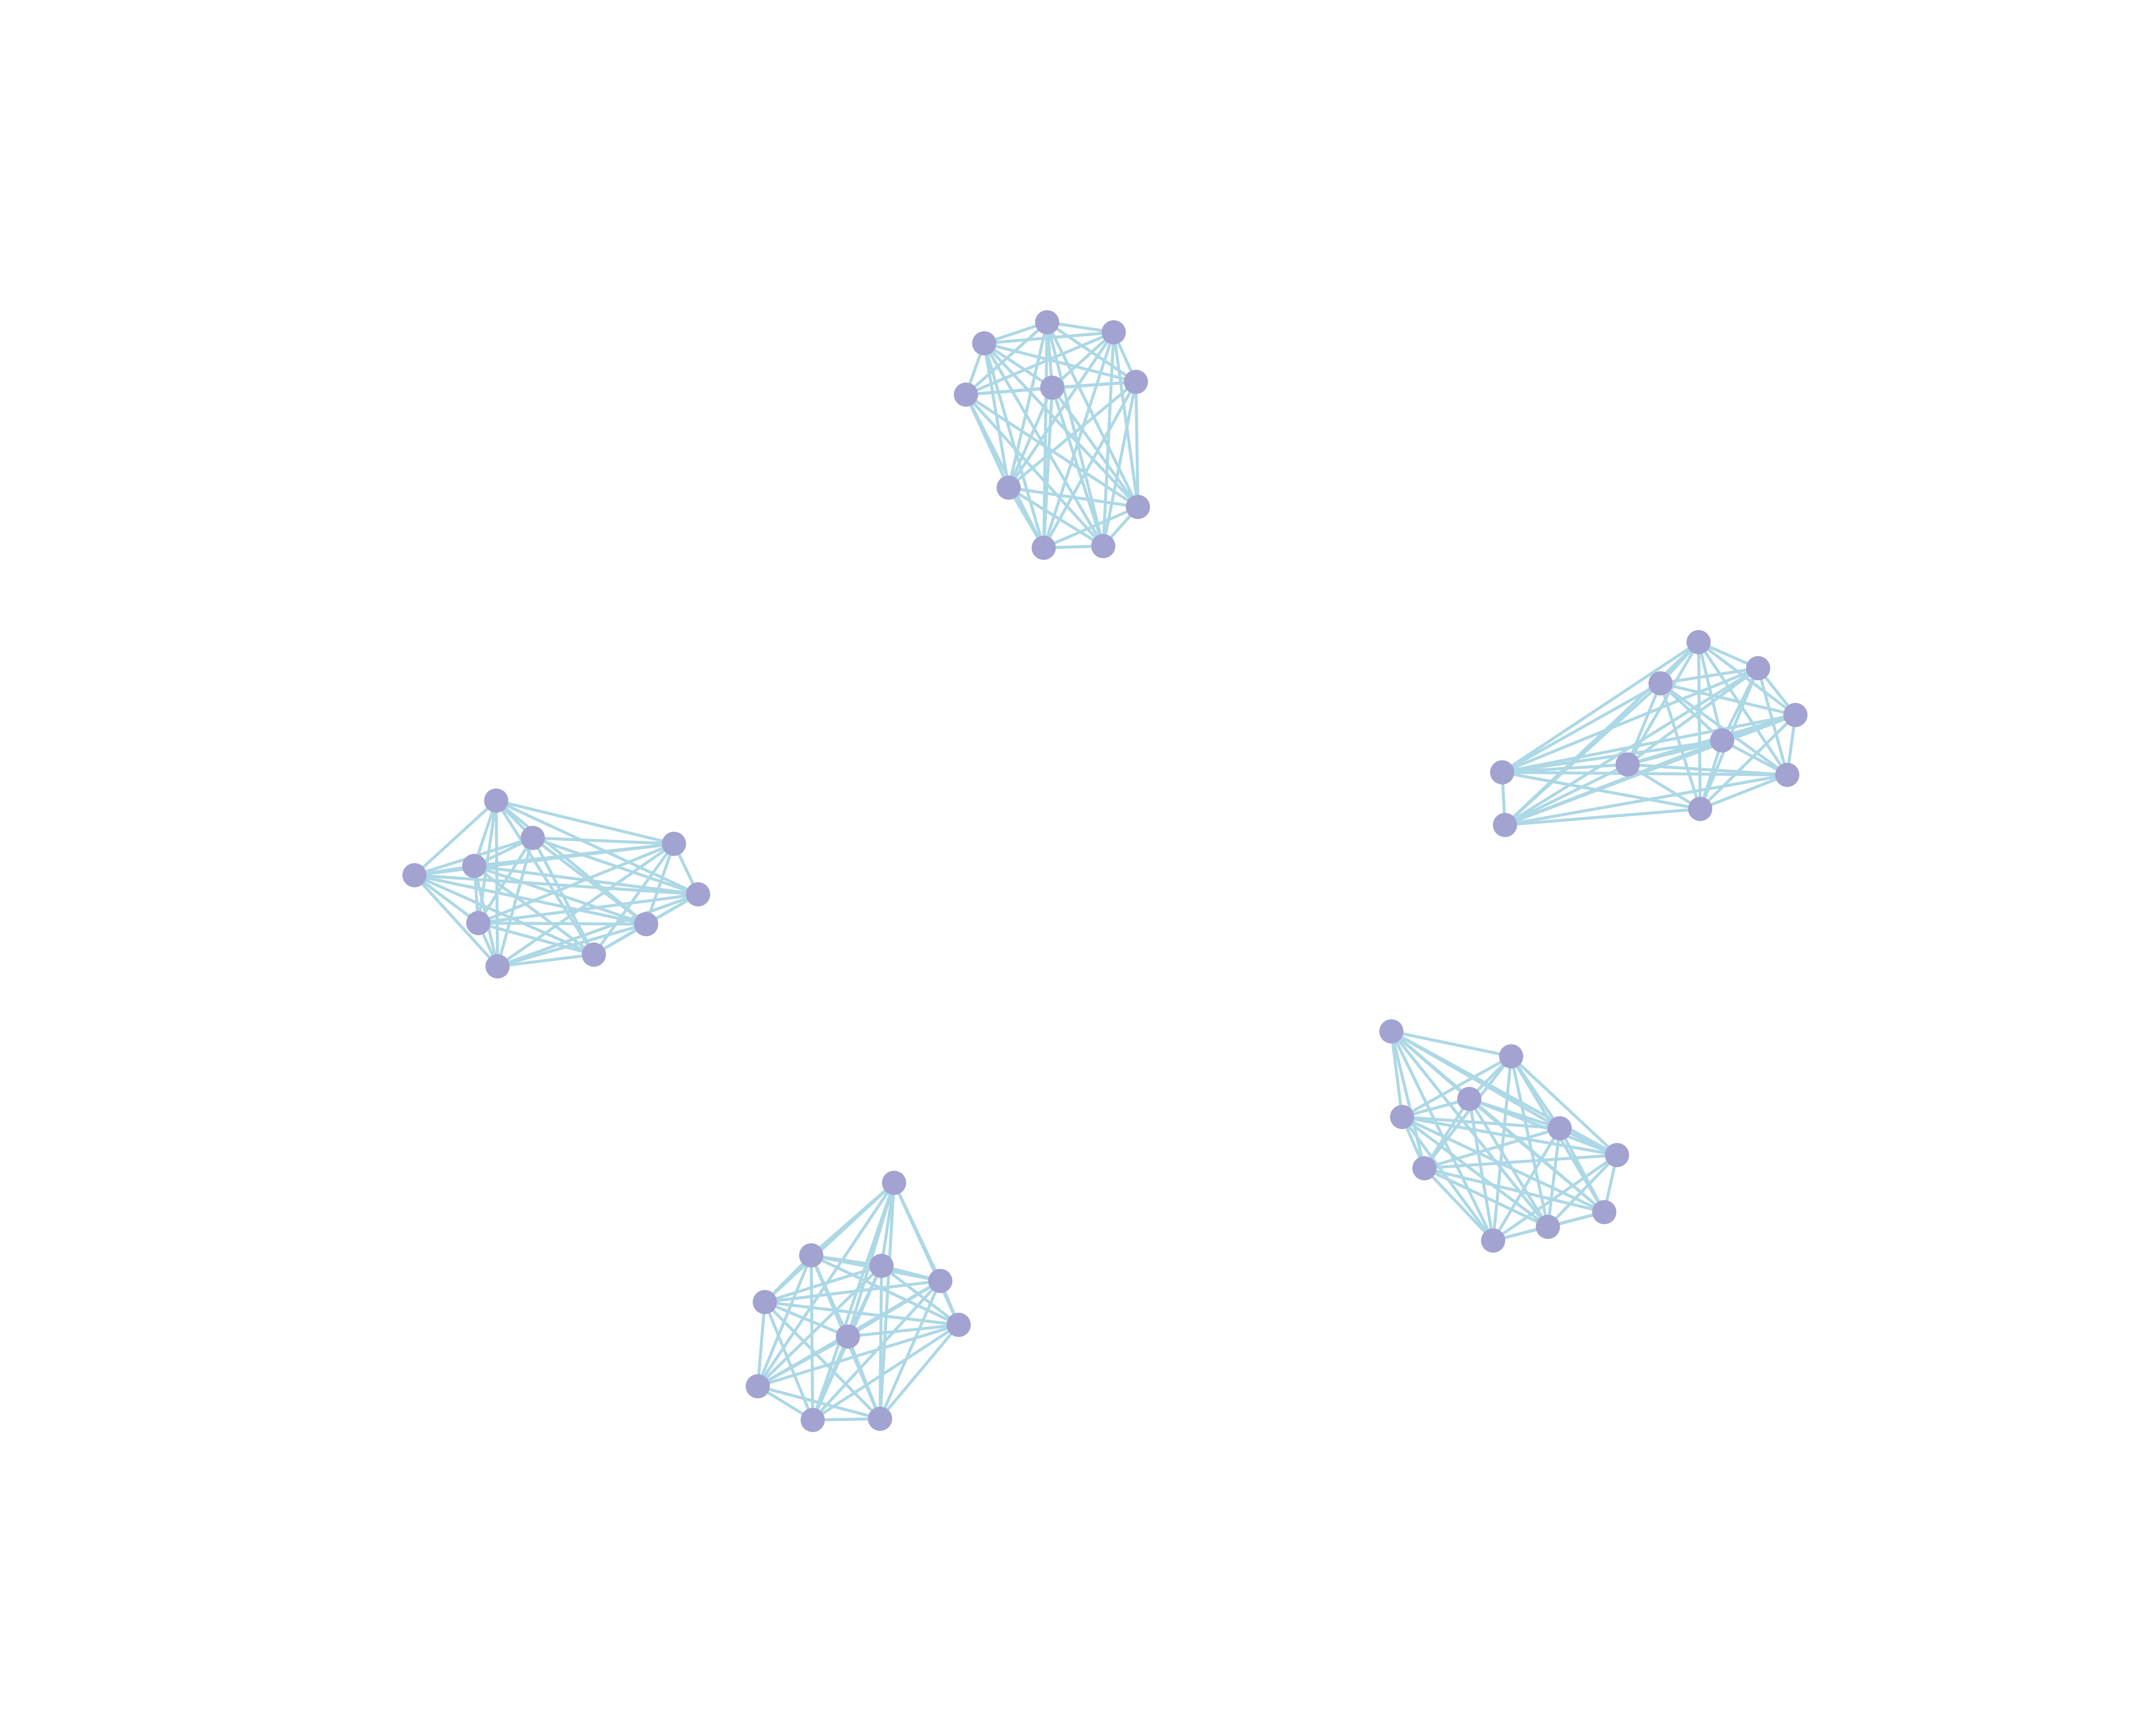
\includegraphics[width=\textwidth]{Graphics/ToyModelResults/Caveman_resluts/BeforeRicciFlow.png}
        \caption{Initial Caveman graph}
        \label{fig:caveman_initial}
    \end{subfigure}
    \hfill
    \begin{subfigure}[b]{0.45\textwidth}
        \centering
        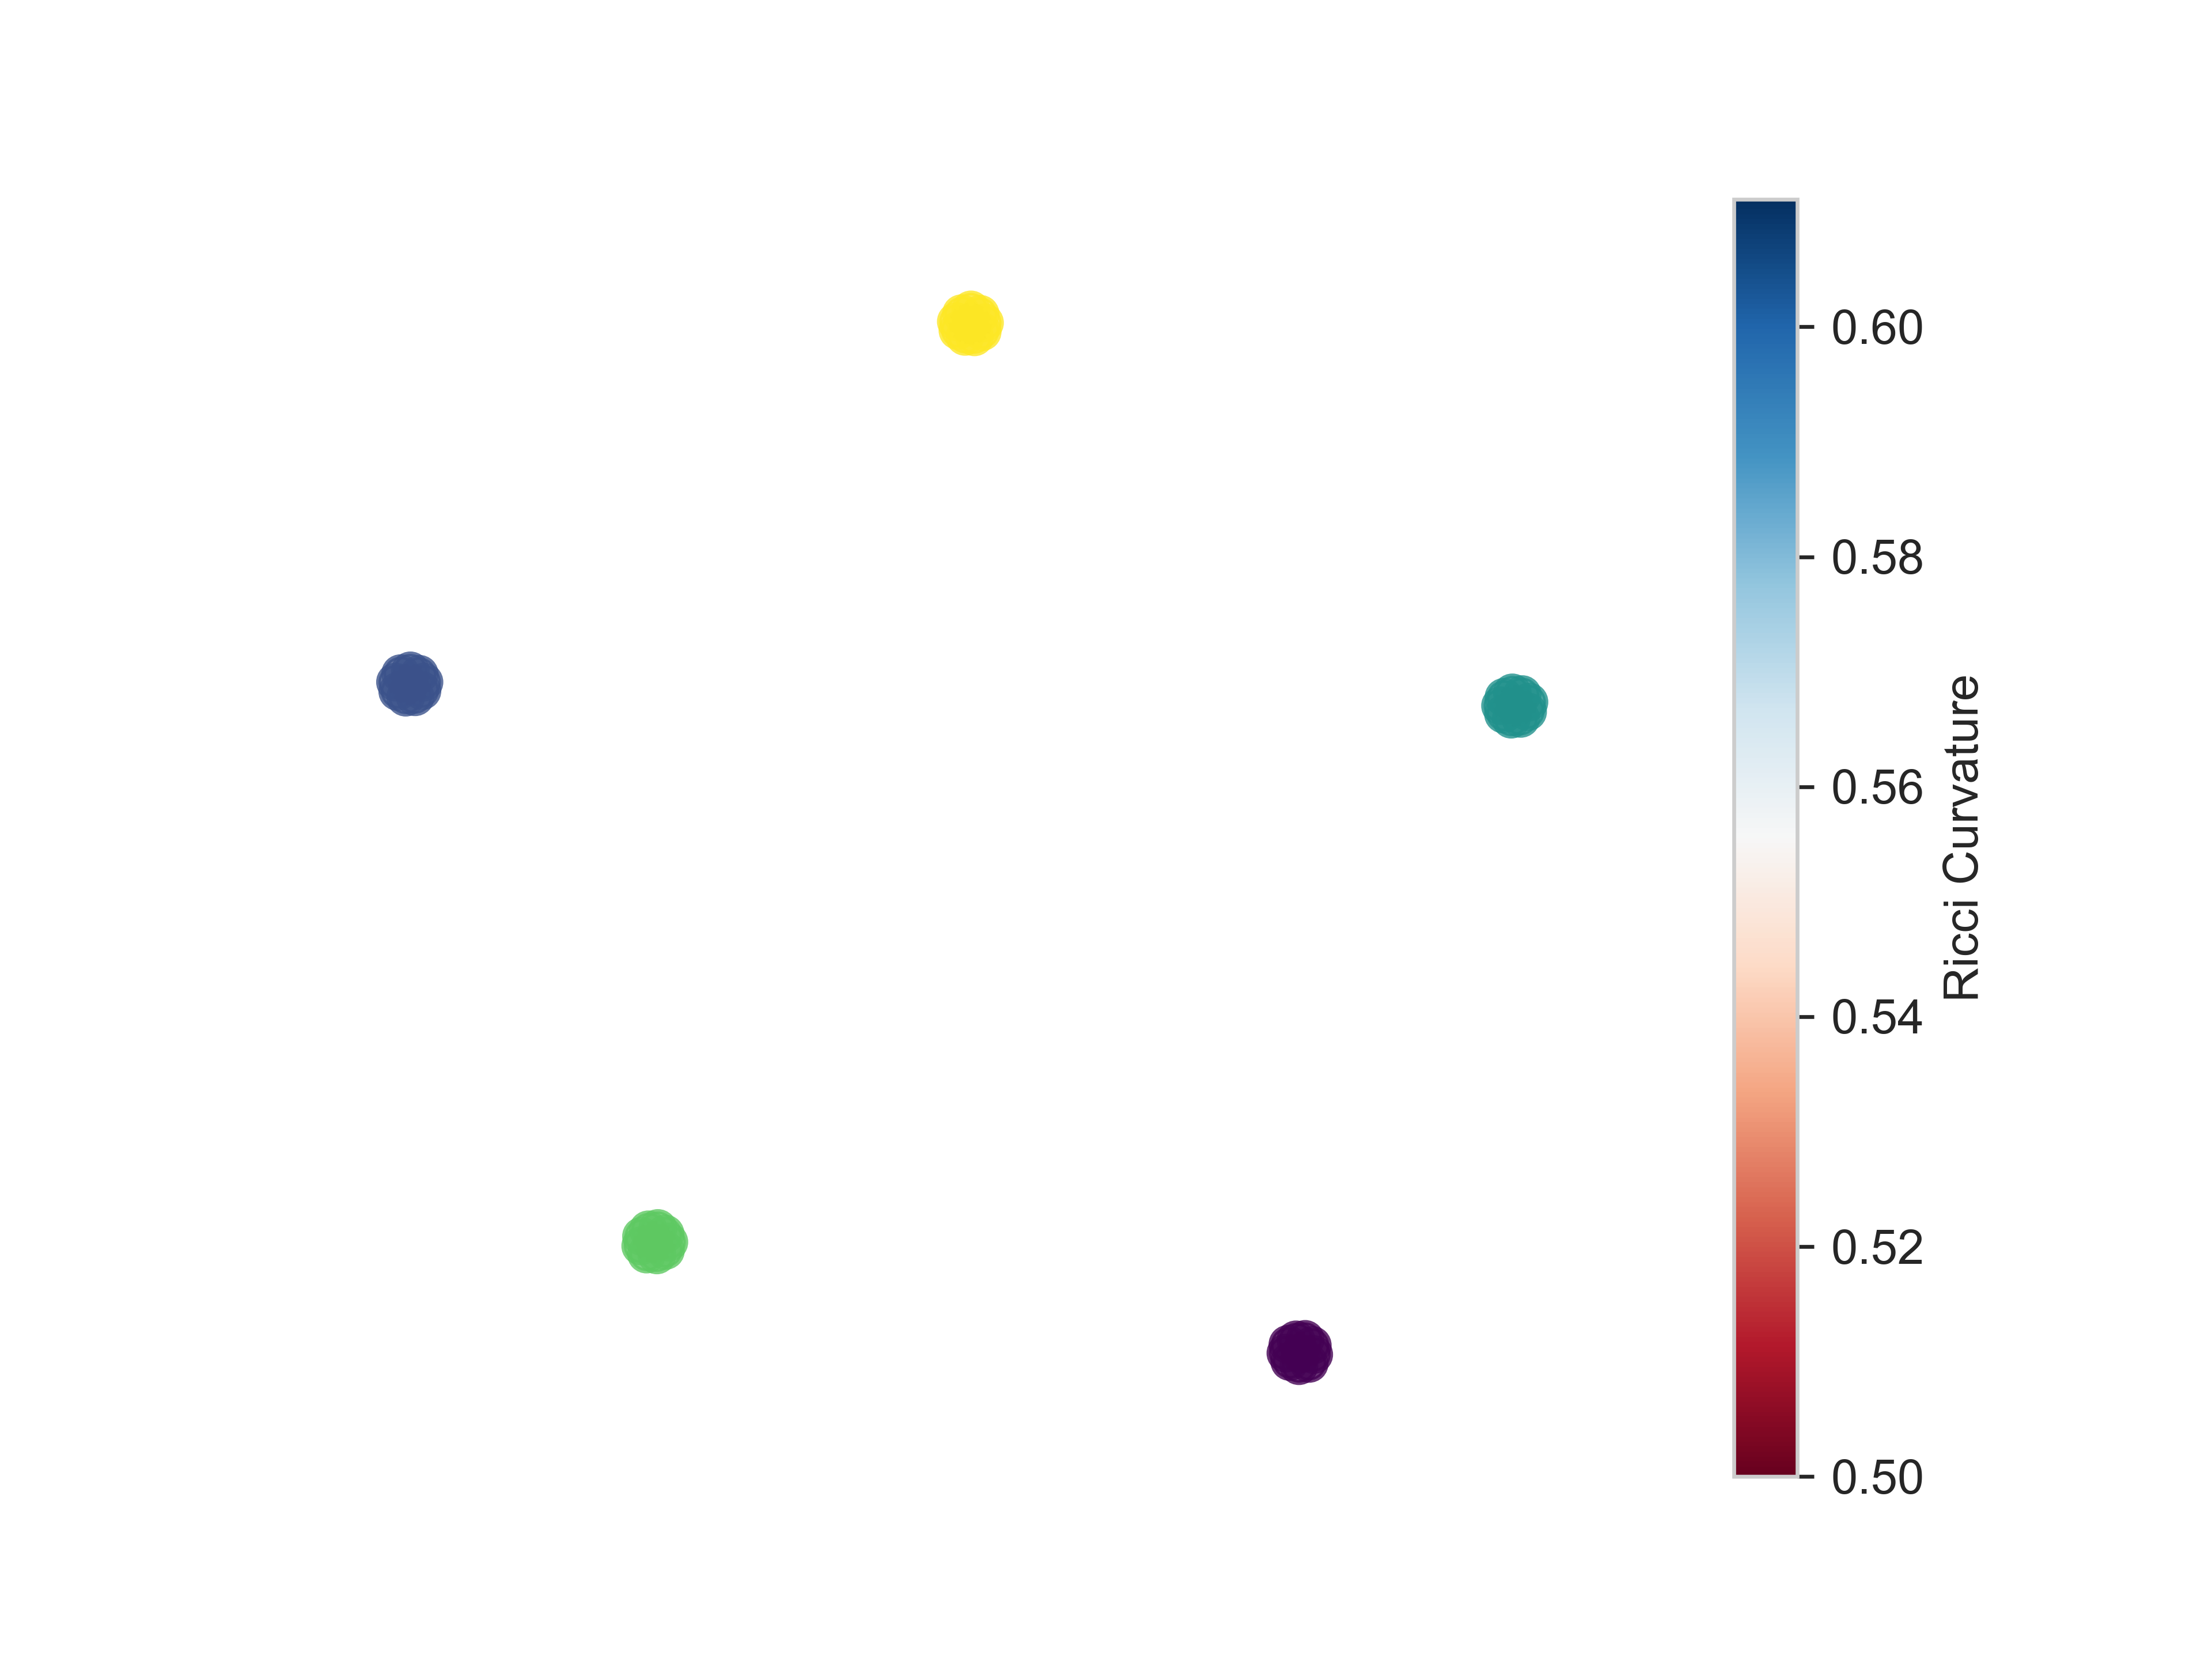
\includegraphics[width=\textwidth]{Graphics/ToyModelResults/Caveman_resluts/Communities.png}
        \caption{Detected communities}
        \label{fig:caveman_result}
    \end{subfigure}
    \caption{Comparison of the initial Caveman graph and the community detection result.}
    \label{fig4}
\end{figure}